\chapter{Fitness Estination}

This chapter explains a proposed strategy to calculate the fitness of the
individual in a web-based interactive evolutionary computation applications
using fuzzy logic. Before showing our strategy, it is necessary to explain how
the individual evaluation is made in the EvoDrawing application. The figure
\ref{fig:UI_ED} shows the user interface where the user interacts with the
application. The main goal of this interaction is the individuals evaluation,
the first action of the user, in order to evaluate, is to login through a social
platform account in this particular case Facebook \cite{facebook}, in order to have
different futures as a collection creation, store individual in a collection,
already explained in the previous chapter. The evaluation takes place through a
five star rate selection by the user; this rate represents the degree of user
preference for an individual. The application keeps the record of every user
activity using the activities stream standard [14]. In these particular case the
activities represents the user experience.

\begin{figure*}
\captionsetup{justification=centering,margin=2cm}
\centering
\setlength\fboxsep{0pt}
\setlength\fboxrule{0.7pt}
\fbox{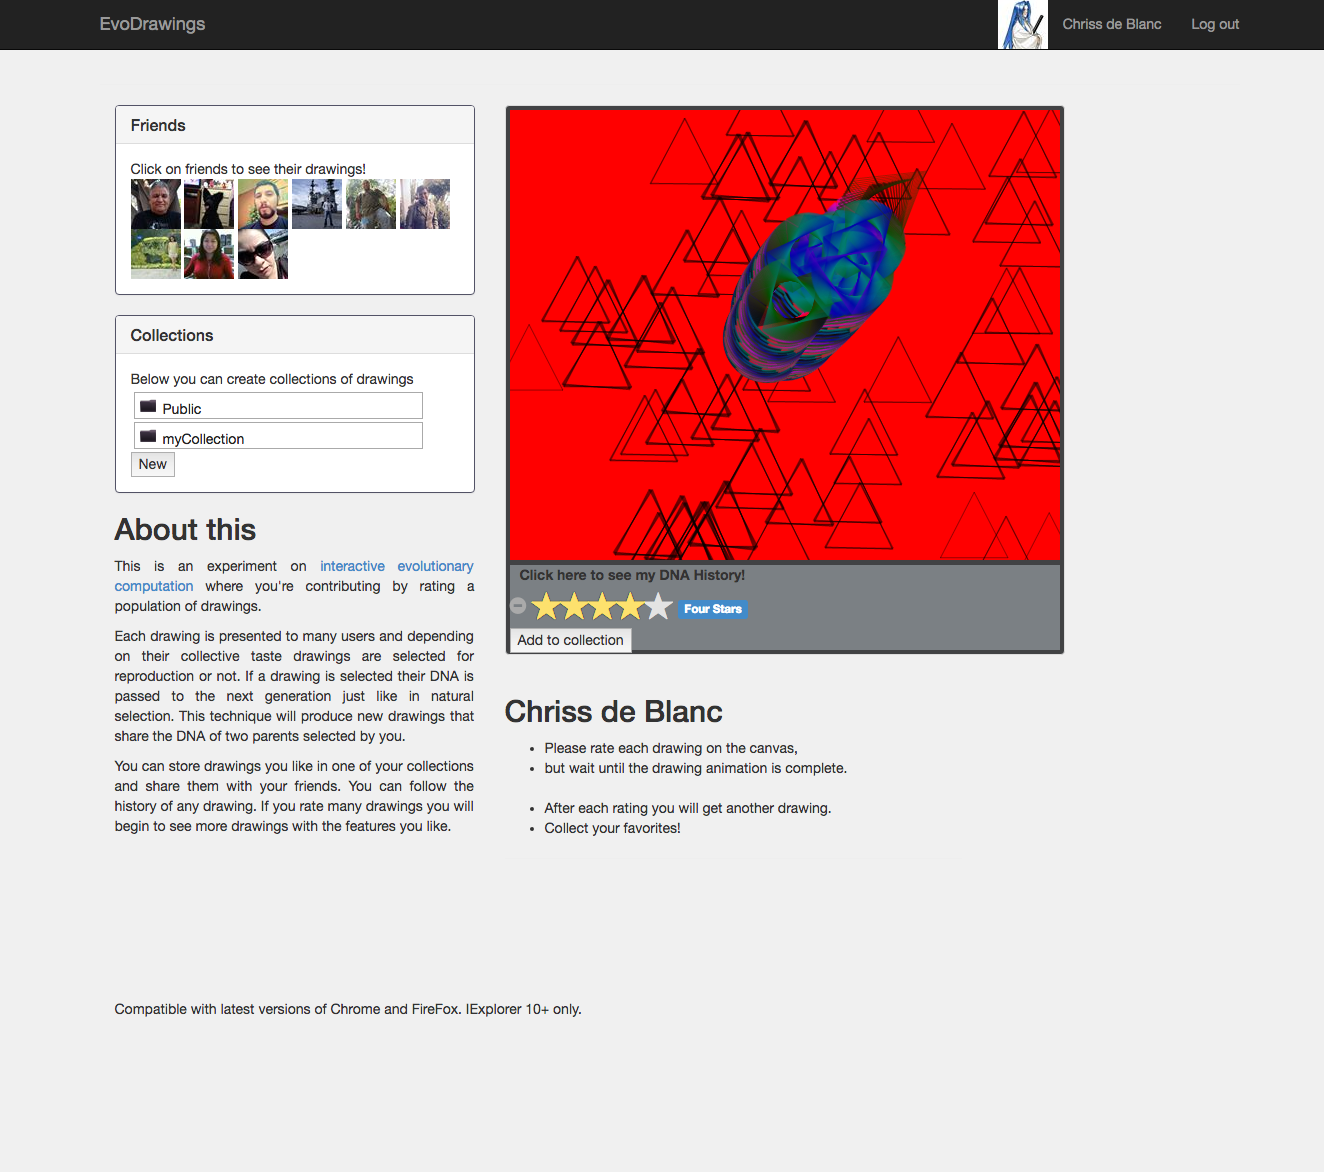
\includegraphics[width=12cm,height=10cm,keepaspectratio]{img/UI_ed01.png}}
\caption{User interface ED01.}
\label{fig:UI_ED}
\end{figure*}

In this research we propose the using of fuzzy logic[10] in order to obtain a
difuzzify value to be used to calculate the individual fitness trough a fitness
function expression. It is used by modeling a fuzzy Mamdani type inference
system [5] [6] as figure \ref{fig:fis01} shown. This model was designed empirically.
The model consists of two input variables, which are the preference and the
experience of the user as well as an output that we called fuzzy rate. The first
one has 3 linguistic variables, which are low, medium and high, representing the
preference with triangular membership functions over a range of 1 to 5. The
second one also has three linguistic variables, which are low, medium and high
representing the experience with triangular membership functions over a range of
1 to 100. Finally we have the output consisting of three linguistic variables
bad, normal and good represent-ing the fuzzy rate with triangular membership
functions in a range of 1-100.

\begin{figure*}
\captionsetup{justification=centering,margin=2cm}
\centering
\setlength\fboxsep{0pt}
\setlength\fboxrule{0.7pt}
\fbox{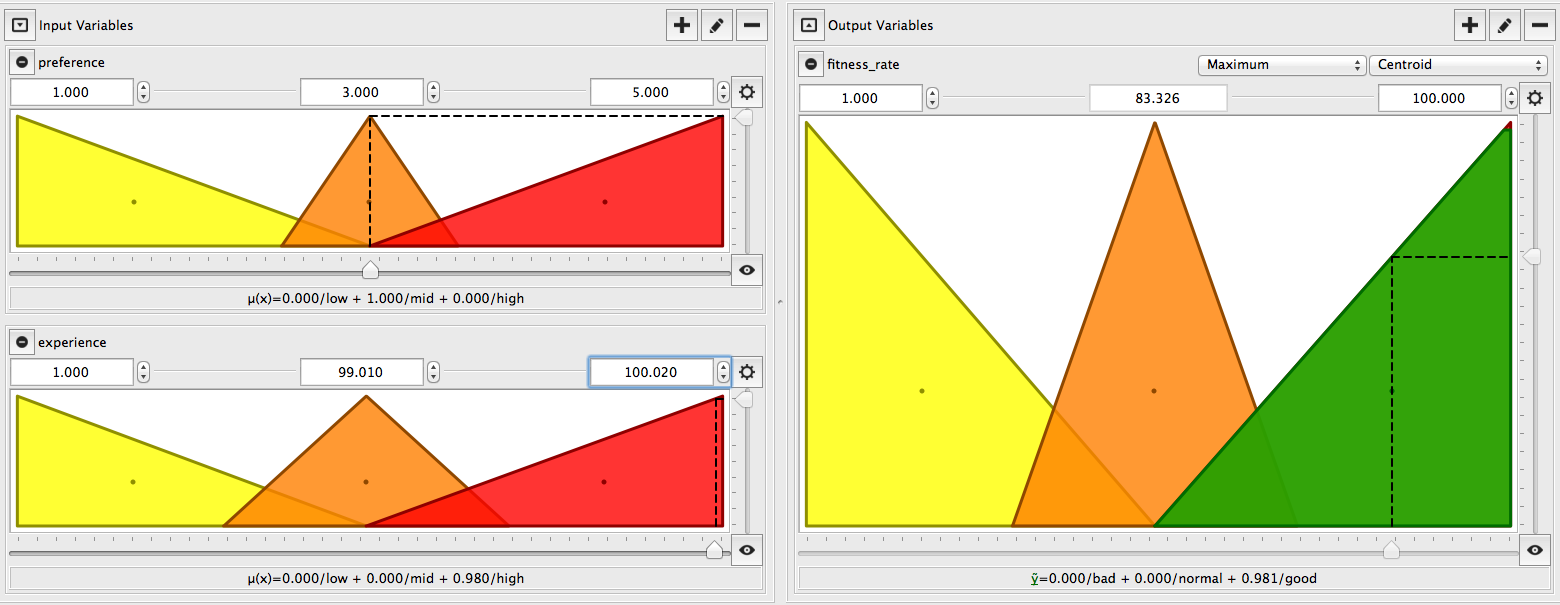
\includegraphics[width=12cm,height=10cm,keepaspectratio]{img/fuzzy_system_2_1.png}}
\caption{Fuzzy System Mamdani Type.}
\label{fig:fis01}
\end{figure*}

Below we show the rules IF-THEN of the fuzzy system:

\begin{enumerate}
	\item \textit{If \textbf{preference} is low and
		\textbf{experience} is low then \textbf{fuzzy\_rate} is bad.}
	\item \textit{If \textbf{preference} is mid and
		\textbf{experience} is low  then \textbf{fuzzy\_rate} is bad.}
	\item \textit{If \textbf{preference} is high and
		\textbf{experience} is low  then \textbf{fuzzy\_rate} is normal.}
	\item \textit{If \textbf{preference} is low and
		\textbf{experience} is mid then \textbf{fuzzy\_rate} is bad.}
	\item \textit{If \textbf{preference} is mid and
		\textbf{experience} is mid  then \textbf{fuzzy\_rate} is normal.}
	\item \textit{If \textbf{preference} is high and
		\textbf{experience} is mid  then \textbf{fuzzy\_rate} is good.}
	\item \textit{If \textbf{preference} is low and
		\textbf{experience} is high then \textbf{fuzzy\_rate} is normal.}
	\item \textit{If \textbf{preference} is mid and
		\textbf{experience} is high  then \textbf{fuzzy\_rate} is good.}
	\item \textit{If \textbf{preference} is high and
		\textbf{experience} is high  then \textbf{fuzzy\_rate} is good.}

\end{enumerate}

These rules will give us a fuzzy rate value result, this is the value need it to
be defuzzify by the centroid method in order to be used in our fitness
expression, given by equation\ref{eq:fitfunc_02}. This expression is responsible
to represent the individual fitness.

\begin{equation}\label{eq:fitfunc_02}
\displaystyle fitness=\frac{\sum_{i=0}^{n}x_{i}+f(y_{i})}{\sum_{i=0}^{n}f(y_{i})}
\end{equation}

Where $n$ represents  the number of  users that  have given an evaluation of the
individual, $x$ is the rate of preference for the  individual  given by  the user,
$y$ is a function that calls the fuzzy system in order to have the fuzzy rate.
This function needs $x$ and the user experience level. The user experience level
is given  by the  total activities that user have at the moment. In each
activity we assign the score, for example if the user log in (join) to the
application we assign 5 points, if the user evaluates (likes) an individual we
give 3 points, etc; in figure 5 shows the flow for assigning fitness to
the individual.
